\section{Methods}

\begin{frame}
	\frametitle{Methods}
	\framesubtitle{Data representation}
	\begin{itemize}
		\item Treat every image as a 3D-tensor (RGB)
			\begin{itemize}
				\item Repeat the value of grayscale images three times
				\item Colorized are handled as the original tensors
			\end{itemize}
		\item Original data has 14 labels, we used 15
			\begin{itemize}
				\item Extra one for the unclassified images
				\item One-hot encoded labels
			\end{itemize}
	\end{itemize}
\end{frame}


\begin{frame}
	\frametitle{Methods}
	\framesubtitle{Data processing}
	\begin{itemize}
		\item Read images in batches of size 2000
		\begin{itemize}
			\item Helps to avoid filling the RAM
		\end{itemize}
		\item Normalize the pixel values between $[0.0, 1.0]$
		\item For every batch augmenting the data
		\begin{itemize}
			\item Provided by Keras
			\item Centerify, shear, zoom, rotate and flip
			\item To get more variation and samples from classes with few labels
		\end{itemize}
	\end{itemize}
\end{frame}

\begin{frame}
	\frametitle{Methods}
	\framesubtitle{Class weights 1/2}
	\begin{itemize}
		\item Classes are very unbalanced
		\begin{figure}[h]
		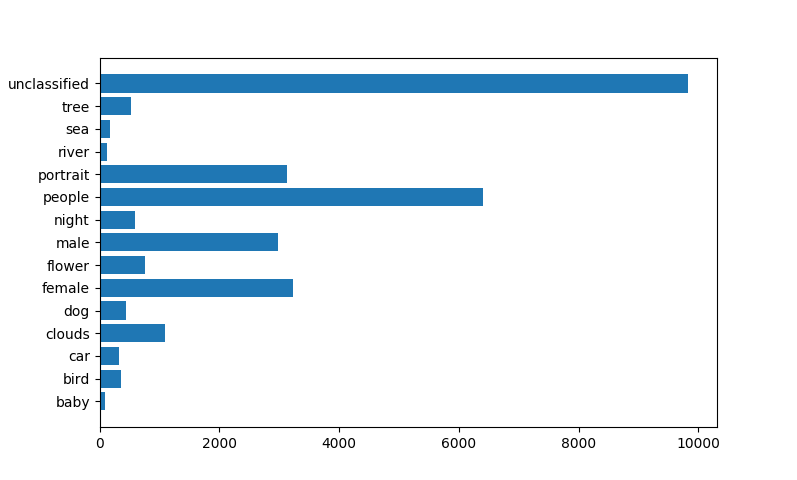
\includegraphics[height=0.6\textheight]{images/label_distribution.png}
		\caption{Class distribution}
		\end{figure}
	\end{itemize}
\end{frame}

\begin{frame}
	\frametitle{Methods}
	\framesubtitle{Class weights 2/2}
	\begin{itemize}
			\item We tackled this problem by custom weights per class
			\begin{itemize}
				\item Giving them at training phase
			\end{itemize}
		\end{itemize}
	\begin{block}{Class weight function}
		$W(c_i;\lambda) = \ln\left(\dfrac{\lambda \sum_{c}|c|}{|c_i|}\right)$
	\end{block}
\end{frame}

\begin{frame}
	\frametitle{Methods}
	\framesubtitle{Topology}
	\begin{itemize}
		\item Thing1
		\item Thing2
	\end{itemize}
\end{frame}

\begin{frame}
	\frametitle{Methods}
	\framesubtitle{Loss function}
	\begin{itemize}
		\item Thing1
		\item Thing2
	\end{itemize}
\end{frame}

\begin{frame}
	\frametitle{Methods}
	\framesubtitle{Validation}
	\begin{itemize}
		\item Thing1
		\item Thing2
	\end{itemize}
\end{frame}